\chapter{METODOLOGI}
\label{chap:desainimplementasi}

% Ubah bagian-bagian berikut dengan isi dari desain dan implementasi

Pada bab metodologi akan dijelaskan mengenai bagaimana cara sistem ini
dibuat. Tujuan dari sistem ini adalah membuat model klasifikasi
tingkat kantuk seseorang dengan parameter EAR dan MAR menggunakan IndRNN
dengan \emph{output} 3 kelas berbeda.

\section{Metode yang digunakan}

% Contoh input gambar dengan format *.jpg
\begin{figure} [ht] \centering
      % Nama dari file gambar yang diinputkan
      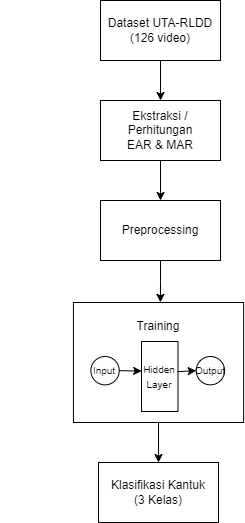
\includegraphics[scale=0.75]{gambar/metodologi.png}
      % Keterangan gambar yang diinputkan
      \caption{Diagram alur model}
      % Label referensi dari gambar yang diinputkan
      \label{fig:metodologi}
\end{figure}

% Contoh penggunaan referensi dari gambar yang diinputkan
Pada diagram yang tertera di Gambar \ref{fig:metodologi}. Didapatkan proses sebagai berikut:
\subsection{Pengumpulan Data}
Dataset UTA-RLDD digunakan sebagai sumber data input. Setiap video dalam kumpulan data ini memiliki perkiraan durasi
10 menit. Pengumpulan data dilakukan secara diseleksi secara manual. Dataset UTA-RLDD memiliki subjek video yang sangat beragam mulai
dari jenis kelamin, etnis, kegiatan yang dilakukan, ukuran video, keberadaan rambut wajah, dan pemakaian kacamata.
Terdapat beberapa video yang tidak bisa terbuka sehingga perlu dilakukan penyaringan data. Adapun kriteria dari
data yang dipilih adalah:
\begin{enumerate}[nolistsep]
      \item Video memiliki fps mendekati 30fps.
      \item Video memiliki jumlah frame diatas 16200.
      \item Video memiliki pencahayaan yang baik.
\end{enumerate}

\subsection{Ekstraksi Fitur}

\begin{figure} [ht] \centering
      % Nama dari file gambar yang diinputkan
      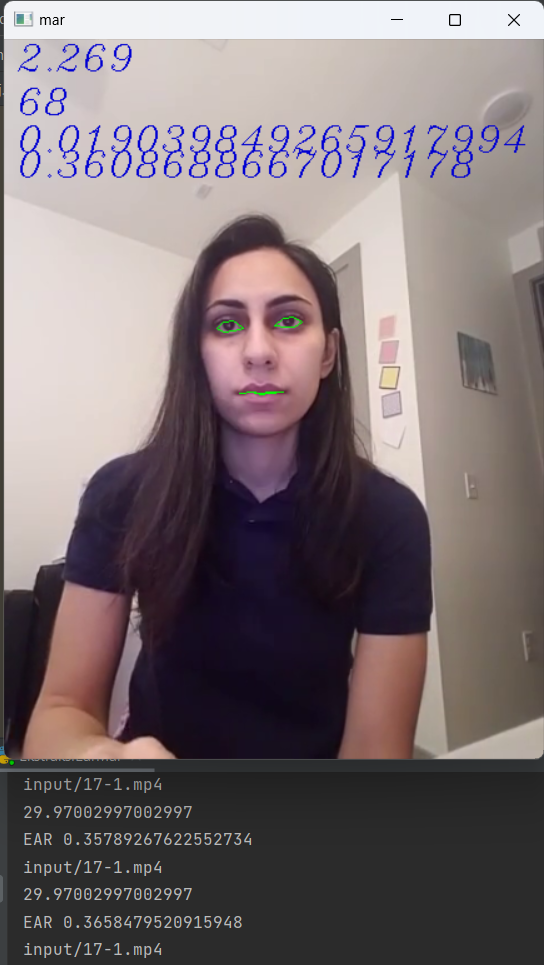
\includegraphics[scale=0.65]{gambar/ekstraksi.png}
      % Keterangan gambar yang diinputkan
      \caption{Proses ekstraksi nilai EAR dan MAR}
      % Label referensi dari gambar yang diinputkan
      \label{fig:ekstraksi}
\end{figure}

Ekstraksi fitur pada tiap video yang telah terpilih dilakukan secara lokal dengan bantuan IDE PyCharm edisi 2021.3.3.
Library Dlib menggunakan pendekatan berbasis fitur untuk mendeteksi landmark wajah. Algoritma pada library Dlib menggunakan
metode Histogram of Oriented Gradients (HOG) yang dikombinasikan dengan \emph{Support Vector Machines} (SVM) untuk mengenali pola wajah.
Deteksi wajah ini akan menghasilkan kotak pembatas (\emph{bounding box}) yang mengelilingi wajah dalam video. Setelah mendeteksi wajah,
langkah selanjutnya adalah menggunakan prediktor landmark Dlib untuk mengidentifikasi titik-titik landmark pada wajah.

Prediktor landmark menggunakan metode regresi untuk memprediksi koordinat titik landmark pada wajah berdasarkan fitur-fitur yang terlihat
dalam gambar. Prediktor ini mengambil gambar wajah yang terdeteksi sebagai input dan menghasilkan koordinat landmark yang sesuai.
Koordinat 68 titik landmark ini mencakup fitur-fitur seperti mata, hidung, mulut, dan sebagainya \parencite{13}. Setiap titik landmark
direpresentasikan oleh sepasang koordinat (x, y) yang menunjukkan posisinya dalam gambar seperti gambar \ref{fig:ekstraksi}.

Fitur-fitur yang diekstraksi pada tiap video yaitu nilai dari EAR dan MAR. Rumus \ref{eq:EAR} digunakan untuk mendapatkan
nilai EAR serta rumus \ref{eq:MAR} untuk mendapatkan nilai MAR. Rumus-rumus tersebut kemudian dimasukkan ke dalam program
sehingga menghasilkan data berupa csv yang berisi nilai EAR dan MAR dari tiap frame dalam setiap video. Nilai dari EAR dan MAR,
akan didapatkan pada tiap frame berdasarkan waktu.

\subsection{\emph{Preprocessing Data}}
Preprocessing data dilakukan menggunakan GoogleColab. Preprocessing data dilakukan untuk untuk meningkatkan kualitas data, mengurangi noise, dan membuat data siap digunakan untuk
pelatihan model. Tahapan preprocessing data yang telah dilakukan dalam penelitian ini adalah mengatasi data kosong, penyetaraan jumlah
data dan pemberian label, melakukan standarisasi data, serta melakukan kostumisasi pada data sehingga cocok digunakan untuk IndRNN.
Tahapan-tahapat tersebut dapat digambarkan menjadi gambar \ref{fig:preprocessing}:

% \newpage
\begin{figure} [ht] \centering
      % Nama dari file gambar yang diinputkan
      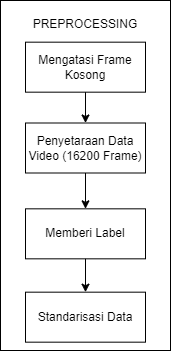
\includegraphics[scale=0.8]{gambar/preprocessing.png}
      % Keterangan gambar yang diinputkan
      \caption{Diagram Preprocessing Data}
      % Label referensi dari gambar yang diinputkan
      \label{fig:preprocessing}
\end{figure}

\newpage
\begin{enumerate}[nolistsep]
      \item Interpolasi Linear

            Terdapat beberapa frame dari video yang landmark wajahnya
            tidak terdeteksi sehingga menyebabkan koordinat landmark wajah bernilai NaN.
            Interpolasi linear diperlukan untuk memperkirakan nilai di antara dua titik data yang diketahui.
            Interpolasi linear mengacu pada estimasi nilai di antara dua titik data yang diberikan
            berdasarkan garis lurus yang menghubungkan kedua titik tersebut. Konsep dasar interpolasi
            linear adalah menggunakan persamaan garis untuk memperkirakan nilai di antara dua titik data.
            Persamaan garis linear dinyatakan sebagai persamaan \ref{eq:interpolasi}:

            \begin{equation}
                  % Label referensi dari persamaan yang dibuat
                  \label{eq:interpolasi}
                  % Baris kode persamaan yang dibuat
                  y = mx + c
            \end{equation}

            Setelah nilai koordinat tiap frame tidak ada yang bernilai NaN maka nilai EAR dan MAR dapat kembali dihitung
            menggunakan hasil interpolasi koordinat titik-titik yang ada pada mata dan mulut dengan memasukkannya
            pada rumus \ref{eq:EAR} dan rumus \ref{eq:MAR}.

      \item \emph{Data Balancing} dan \emph{Labeling}

            Jumlah frame yang ada pada tiap video tidaklah sama oleh karena itu diperlukan pemotongan jumlah frame pada tiap video
            sehingga jumlah framenya dapat seragam yaitu 16200 frame tiap video. Ketika jumlah frame tiap video sudah seragam maka
            diberikanlah label yang sama pada tiap frame dalam satu video. Data-data tersebut kemudian dijadikan dalam satu csv
            sehingga lebih mudah untuk melakukan tahap preprocessing data selanjutnya.

      \item Normalisasi Standard Scaler

            Metode normalisasi standard scaler umum digunakan dalam preprocessing data. Tujuannya adalah untuk
            mentransformasikan data sehingga memiliki mean (rerata) nol dan deviasi standar satu. Normalisasi standard
            scaler dapat membantu meningkatkan performa model serta menghilangkan perbedaan skala antar fitur dalam dataset.
            Dengan demikian, semua fitur akan memiliki skala yang serupa, yang memudahkan perbandingan dan interpretasi data.
            Normalisasi data dengan fungsi Standard Scaler dapat diakses melalui library sklearn. Cara kerja dari normalisasi
            ini adalah mengganti nilai tersebut dengan nilai yang dihasilkan melalui rumus \ref{eq:StandardScaler}.

      \item Sliding Window

            \begin{figure} [ht] \centering
                  % Nama dari file gambar yang diinputkan
                  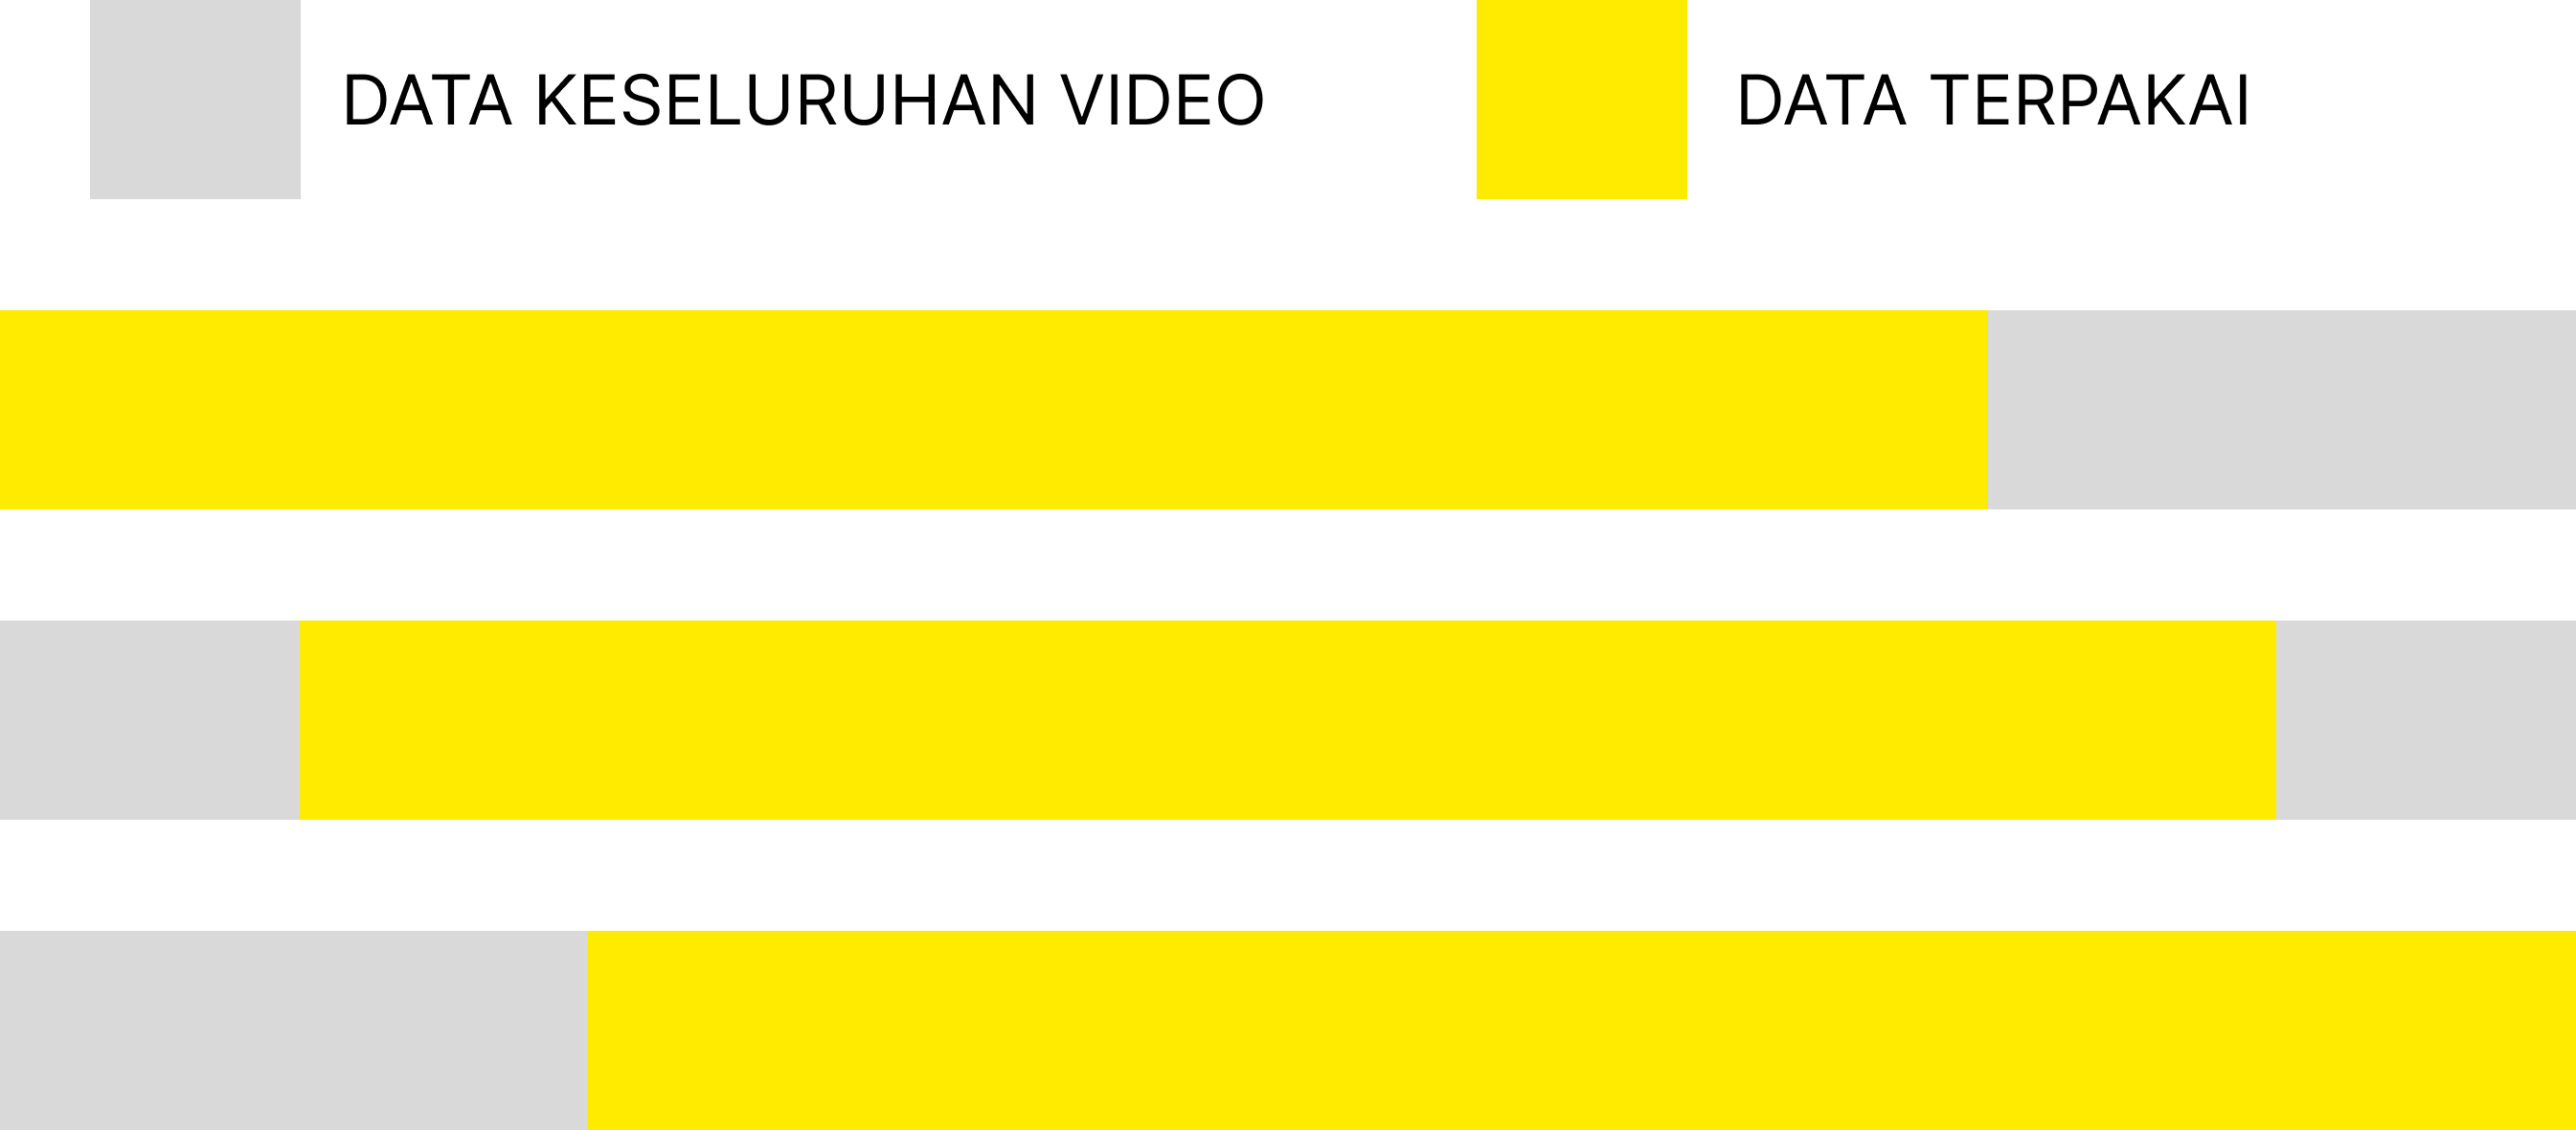
\includegraphics[scale=0.15]{gambar/PotongData.png}
                  % Keterangan gambar yang diinputkan
                  \caption{Ilustrasi pemotongan data}
                  % Label referensi dari gambar yang diinputkan
                  \label{fig:potong}
            \end{figure}
            Sebelum data dimasukkan ke sliding window, data terlebih dahulu dipisahkan menjadi data training dan data validasi atau
            testing. Sliding window digunakan sebagai teknik pemrosesan data untuk mempersiapkan data masukan yang lebih
            sesuai dengan kebutuhan model.  Metode sliding window digunakan karena masukan feature bersifat kontinu dan dalam satu
            feature terdapat banyak nilai yang tersimpan di dalam array.

            Dilakukan augmentasi pada data training dengan melakukan pemotongan data pada titik acu yang berbeda. Jumlah data bervariasi
            dalam tiap video namun data yang diambil sebagai masukan model berjumlah 16200. Oleh karena itu dilakukan pemotongan dengan
            titik acu yang berbeda untuk menghasilkan data augmentasi. Pemotongan dilakukan dengan variasi dari awal data, dari tengah data, dan dari akhir data  yang dapat diilustrasikan
            seperti gambar \ref{fig:potong}.
\end{enumerate}

\subsection{\emph{Training Data}}
Pada proses klasifikasi yang menggunakan IndRNN nilai EAR dan MAR digunakan se-
bagai feature untuk proses training. Untuk output-nya sendiri akan terdiri dari 3 kelas yang
mengacu pada skala kantuk karolinska. 3 kelas tersebut terdiri dari: Kelas pertama (Waspada)
yaitu terdiri dari label kelas KSS 1 sampai 5 ( Amat Sangat Terjaga, Sangat Terjaga, Terjaga,
Sedikit terjaga, Tidak Terjaga namun Tidak ada Tanda Mengantuk), Kelas kedua (Kewaspadaan
Rendah) yaitu terdiri dari label kelas KSS 6 dan 7 ( Sedikit Mengantuk dan Mengantuk, perlu
sedikit usaha untuk terjaga), Kelas ketiga (Mengantuk) yaitu terdiri dari label kelas KSS 8 dan
9 (Mengantuk, perlu usaha untuk terjaga dan Sangat mengantuk, perlu usaha lebih untuk tetap
terjaga). Model klasifikasi dibuat menggunakan IndRNN sebagai klasifikatornya.

Berikut adalah gambaran arsitektur IndRNN yang digunakan:

\newpage
\begin{figure} [H] \centering
      % Nama dari file gambar yang diinputkan
      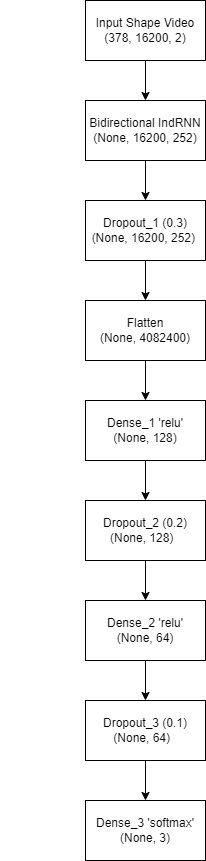
\includegraphics[scale=0.7]{gambar/arsitekturmodel.png}
      % Keterangan gambar yang diinputkan
      \caption{Arsitektur Model Klasifikasi IndRNN}
      % Label referensi dari gambar yang diinputkan
      \label{fig:arsitekturmodel}
\end{figure}

\begin{enumerate}[nolistsep]
      \item Input: IndRNN menerima input berupa urutan data, seperti urutan waktu dalam bentuk deret waktu atau urutan spasial dalam citra.
            Setiap elemen dalam urutan dianggap sebagai input pada satu waktu tertentu. IndRNN memiliki input yang berpentuk 3 dimensi jika
            pada penelitian yang dilakukan, bentuk input modelnya adalah (353, 16200, 2).

      \item Hidden Units: Setiap unit rekuren dalam IndRNN memiliki \emph{hidden state} atau \emph{output} yang dihasilkan dari pemrosesan input dan
            bobotnya. Hidden state ini merepresentasikan informasi yang dihasilkan oleh unit rekuren pada waktu tertentu. Model klasifikasi
            pada penelitian ini memiliki 126 hidden units.

      \item Weight Matrix: Setiap unit rekuren dalam IndRNN menggunakan \emph{weight matrix} (matriks bobot) yang berkorelasi dengan dirinya sendiri.
            Matriks bobot ini digunakan dalam operasi perkalian untuk menghitung \emph{output} unit rekuren pada waktu tertentu.

      \item Non-linear Activation: Setelah melakukan operasi perkalian dengan input dan bobotnya, output dari setiap unit rekuren umumnya
            melewati fungsi aktivasi non-linear, seperti fungsi ReLU, untuk memperkenalkan sifat non-linearitas dalam jaringan.

      \item \emph{Output}: IndRNN dapat menghasilkan output pada setiap waktu tertentu berdasarkan hidden state dari unit-unit rekuren. \emph{Output} ini
            dapat digunakan untuk klasifikasi kantuk yang menghasilkan 3 jenis kelas berbeda.

\end{enumerate}

Model klasifikasi yang dibuat dengan arsitektur SVM, menggunakan parameter kernel RBF.
Kernel RBF (\emph{Radial Basis Function}) atau juga dikenal sebagai Gaussian kernel adalah
salah satu jenis kernel yang memetakan data ke dalam ruang fitur yang memiliki dimensi tak
terhingga. Kernel RBF memberikan bobot pada setiap titik data berdasarkan jaraknya dari pusat.
Semakin dekat titik data dengan pusat, semakin besar bobotnya. Dalam kernel RBF, bobot jarak
dihitung dengan menggunakan fungsi Gaussian, yang menurun secara eksponensial dengan
jarak. Kernel RBF digunakan untuk memodelkan hubungan non-linear antara fitur-fitur dalam
data. Dengan melakukan pemetaan data ke dalam ruang fitur yang memiliki dimensi tak
terhingga, kernel RBF memungkinkan SVM untuk menemukan hiperplane non-linear yang
dapat memisahkan kelas-kelas data dengan lebih baik.



Berikut merupakan gambaran arsitektur LSTM yang digunakan sebagai model
klasifikasi kantuk:
\begin{figure} [ht] \centering
      % Nama dari file gambar yang diinputkan
      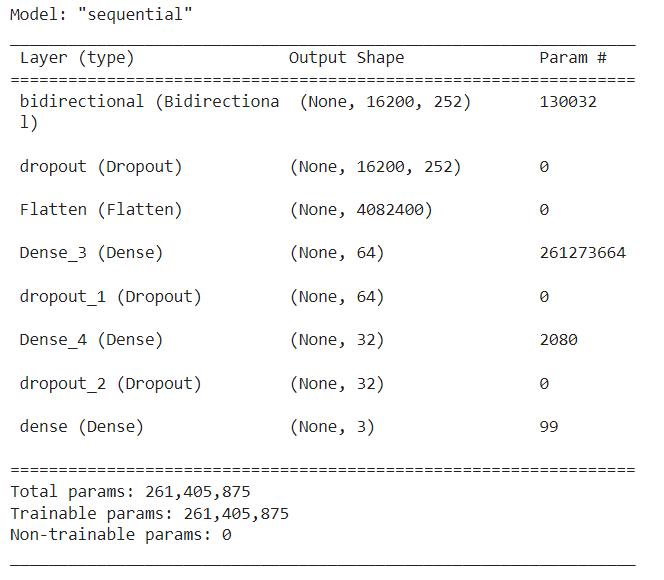
\includegraphics[scale=0.7]{gambar/arsitekturLSTM.png}
      % Keterangan gambar yang diinputkan
      \caption{Arsitektur Model Klasifikasi LSTM}
      % Label referensi dari gambar yang diinputkan
      \label{fig:arsitekturLSTM}
\end{figure}

\newpage
Berikut merupakan tabel hyperparameter yang digunakan untuk membangun model klasifikasi pada penelitian ini:

\begin{longtable}{|c|c|}
      \caption{Pengaturan Hyperparameter Model Klasifikasi}
      \label{tb:Hyperparameter}                             \\
      \hline
      \rowcolor[HTML]{C0C0C0}
      \textbf{Hyperparameter}              & \textbf{Nilai} \\
      \hline
      Arsitektur Model (IndRNN, LSTM, SVM) & 126 unit       \\
      Regularisasi L2                      & 1e-07          \\
      Dropout\_1                           & 0.3            \\
      Dropout\_2                           & 0.2            \\
      Dropout\_3                           & 0.1            \\
      activation                           & ReLu           \\
      output activation                    & softmax        \\
      solver                               & adam           \\
      initial learning rate                & 0.000025       \\
      \hline
\end{longtable}

\begin{enumerate}[nolistsep]
      \item Regularisasi L2

            Regularisasi L2 adalah salah satu metode regularisasi dalam pembelajaran mesin. Tujuan dari digunakannya regularisasi L2
            adalah untuk mengendalikan kompleksitas model dan mencegah overfitting. Regulasi L2 biasa digunakan pada data yang kompleks yang
            menyebabkan kondisi model terlalu "menghafal" data pelatihan dan tidak mampu menggeneralisasi dengan baik pada data yang
            belum pernah dilihat sebelumnya. Regularisasi L2 membantu mencegah overfitting dengan mengurangi bobot yang besar, sehingga
            membatasi kapasitas model untuk "menghafal" data pelatihan dan memaksa model untuk fokus pada pola yang lebih umum dan general.
            Regulasi L2 juga dapat membuat model lebih stabil dan konsisten dengan mengendalikan varians serta mengendalikan kemampuan model
            dengan dengan memberikan penalti pada bobot yang lebih besar, sehingga mendorong model untuk menggunakan representasi yang lebih
            sederhana dan parsial dari data.

      \item Fungsi Aktivasi Non-Linear

            Pada model klasifikasi kantuk dengan IndRNN, ReLU digunakan untuk memperkenalkan sifat non-linearitas dalam jaringan.
            Alasan digunakannya ReLU pada model klasifikasi karena implementasinya sederhana, perhitungan ReLU dapat dijalankan
            secara efisien di perangkat keras seperti GPU. ReLU dapat mengurangi masalah gradien yang cenderung menghilang
            (\emph{vanishing gradient}) saat mengalami backpropagation, terutama pada lapisan-lapisan terdalam. ReLU memungkinkan pelatihan
            model yang lebih cepat dan efisien. Fungsi aktivasi softmax digunakan pada lapisan dense terakhir dengan tujuan
            menghasilkan distribusi probabilitas yang menunjukkan kemungkinan setiap kelas sebagai output dari model.

      \item Optimisasi

            Optimisasi Adam (Adaptive Moment Estimation) adalah algoritma optimasi yang menggabungkan konsep dari optimizer RMSProp dan Momentum
            untuk menghasilkan tingkat konvergensi yang cepat dan efisien. Optimisasi Adam menghitung momen pertama dan kedua dari gradien. Momen
            pertama digunakan untuk mengestimasi kecepatan perubahan bobot, sedangkan momen kedua digunakan untuk mengestimasi kecepatan perubahan
            kecepatan perubahan bobot. Hal ini membantu algoritma untuk menyesuaikan langkah optimisasi berdasarkan gradien yang terkini dan
            mempertimbangkan sejarah gradien sebelumnya. Dengan melakukan penyesuaian learning rate berdasarkan estimasi momen, optimisasi Adam
            mampu menyesuaikan langkah optimisasi dengan lebih baik dan mengurangi dampak dari learning rate yang tidak tepat. Optimisasi Adam
            melibatkan regularisasi untuk mencegah overfitting pada model. Regularisasi dilakukan melalui metode L2 regularization.
            Optimizer Adam digunakan untuk mempercepat dan meningkatkan proses pelatihan model IndRNN, sehingga memungkinkan model
            untuk belajar pola yang lebih kompleks dan akurat dari data sequence yang ada.
\end{enumerate}

\subsection{Evaluasi Model}
Evaluasi model dilakukan untuk untuk memahami dan mengukur performa model dalam melakukan prediksi pada dataset.
Beberapa metrik evaluasi yang umum digunakan adalah Confusion Matrix, Akurasi,
Presisi, Recall, dan F1-Score. Semakin tinggi nilai precision, recall, dan f1 score maka semakin baik performa model. Nilai loss yang
mendekati 0 menandakan hasil probabilitas prediksi mendekati nilai yang benar dan juga sebaliknya. Nilai
yang benar pada confusion matrix dapat diliat dari garis diagonalnya. Tahapan skenario evaluasi model
meliputi beberapa poin berikut:

\begin{enumerate}[nolistsep]
      \item Pengujian Performa Model IndRNN dengan Confusion Matrix
      \item Pengujian Performa Model IndRNN dengan Akurasi, Presisi, Recall, dan F1-Score
      \item Pengujian Performa Model LSTM dengan Confusion Matrix
      \item Pengujian Performa Model LSTM dengan Akurasi, Presisi, Recall, dan F1-Score
      \item Pengujian Performa Model SVM dengan Confusion Matrix
      \item Pengujian Performa Model SVM dengan Akurasi, Presisi, Recall, dan F1-Score
\end{enumerate}

\subsection{Pengujian Model}
Pengujian model digunakan untuk mengetahui kinerja model yang telah dibuat. Pengujian model
dilakukan dengan menggunakan video yang ada pada dataset DROZY. Video yang ada pada dataset
diproses dahulu seperti video yang berasal dari dataset UTA-RLDD sehingga menghasilkan
data yang sesuai. Video yang memiliki jumlah frame yang kurang dari 16200 tidak digunakan
untuk melakukan pengujian model.

\section{Data dan peralatan yang digunakan}
Model klasifikasi kantuk dibangun menggunakan data dari dataset UTA-RLDD serta untuk
menguji model klasifikasi digunakan dataset DROZY. Alat yang dibutuhkan untuk membangun
model ini adalah laptop yang terhubung dengan internet sehingga dapat digunakan untuk mengakses
GoogleColab dan PyCharm.

\subsection{Dataset UTA-RLDD}

\begin{figure} [ht] \centering
      % Nama dari file gambar yang diinputkan
      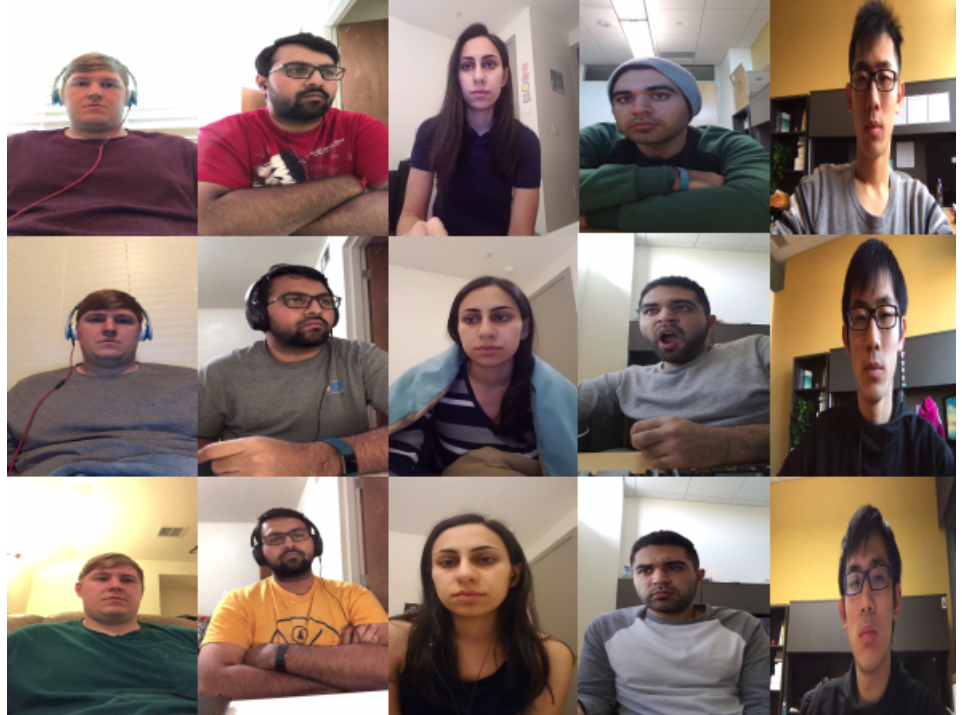
\includegraphics[scale=0.4]{gambar/utarldd.png}
      % Keterangan gambar yang diinputkan
      \caption{Sampel data UTA-RLDD dalam status waspada (baris pertama), waspada rendah (baris kedua), dan mengantuk (baris ketiga) \parencite{14}}
      % Label referensi dari gambar yang diinputkan
      \label{fig:utarldd}
\end{figure}

UTA-RLDD (\emph{The University of Texas at Arlington Real-Life Drowsiness Dataset}) dibuat untuk tugas deteksi kantuk \emph{multi-stages}.
Dataset ini terditi dari 60 subjek sehat (51 laki-laki dan 9 perempuan) dengan usia diatas 18 tahun. Panjang durasi jumlah
video yang ada sekitar 30jam RGB dengan fps hingga 30. Subjek diminta untuk mengambil 3 buah video mereka delam 3 kondisi
kantuk yang berbeda seperti pada gambar \ref{fig:utarldd} dengan durasi masing-masing sekitar 10 menit\parencite{14}. Ketiga kelas tersebut dijelaskan kepada para peserta sebagai
berikut:

1) Waspada: Salah satu dari tiga kondisi pertama yang disorot dalam tabel KSS dengan nilai 1 hingga 3 dimana subyek dalam
keadaan masih waspada dan benar-benar sadar sehingga mereka dapat mengemudi selama berjam-jam dengan mudah.

2) Kewaspadaan Rendah : Memiliki nilai 6 dan 7 dalam tabel KSS dimana ketika beberapa tanda kantuk muncul, atau kantuk
hadir tetapi tidak diperlukan upaya untuk tetap waspada. Subjek mungkin dapat mengemudi dalam kondisi ini tapi tidak dianjurkan.

3) Mengantuk : Keadaan ini berarti subjek harus secara aktif berusaha untuk tidak tertidur dengan nilai 8 dan 9 pada Tabel KSS.

\subsection{Dataset DROZY}

\begin{figure} [ht] \centering
      % Nama dari file gambar yang diinputkan
      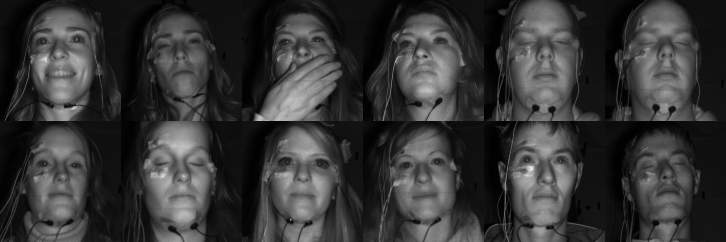
\includegraphics[scale=0.4]{gambar/DROZY.png}
      % Keterangan gambar yang diinputkan
      \caption{Sampel data DROZY \parencite{29}}
      % Label referensi dari gambar yang diinputkan
      \label{fig:DROZY}
\end{figure}

Database DROZY berisi berbagai tipe data yang berhubungan dengan kantuk (sinyal, gambar, dan sebagainya). Sampel data yang ada pada
database DROZY ditunjukkan oleh gambar \ref{fig:DROZY}. Database ini
bertujuan untuk membantu para peneliti untuk melakukan eksperimen, mengembangkan, serta mengevaluasi sistem pada monitoring
kantuk. Data yang ada di DROZY diambil dari 14 partisipan (3 pria, 11 wanita) yang melakukan simulasi berkendara selama
10 menit dalam kondisi kurang tidur yang disebabkan oleh bangun yang berkepanjangan. Untuk setiap subjek, dan untuk setiap
PVT, database berisi data tersinkronisasi waktu dengan sempurna berikut:

1)	Nilai KSS

2)	PVT data

3)	Polysomnography signals

4)	Kinect V2 sensor videos

5)	Face Landmarks (Manual)

6)	Face Landmarks (Otomatis)

7)	Index Interpolasi

\subsection{Peralatan}

Berikut merupakan peralatan yang diperlukan untuk membangun model klasifikasi kantuk dengan menggunakan IndRNN:

\begin{enumerate}[nolistsep]
      \item Laptop yang digunakan untuk mengumpulkan data, training, evaluasi, hingga testing memiliki spesifikasi Intel(R)
            Core(TM) i7-8565U CPU @1.80GHz 1.99 GHz, 16 GB LPDDR3 RAM, 512GB M.2 NVMe PCIe SSD, NVIDIA GeForce MX150 with
            2GB GDDR5 VRAM, Windows 10 Pro 64-bit.
      \item GoogleColab merupakan produk Google research berbasis Cloud yang dapat digunakan secara gratis. Untuk menjalankan
            training model sistem klasifikasi menggunakan IndRNN dibutuhkan TPU serta \emph{Runtime Shape High-RAM} karena jumlah
            data yang ditraining cukup besar.
      \item PyCharm edisi 2021.3.3 digunakan untuk melakukan ekstraksi data secara lokal. PyCharm merupakan IDE (\emph{Integrated Development Environment})
            yang biasa digunakan untuk membangun model \emph{machine learning} yang menawarkan kemudahan untuk membangun \emph{environment} berbeda sesuai
            kebutuhan.

\end{enumerate}

